%%%%%%%%%%%%%%%%%%%%%%%%%%%%%%%%%%%%%%%%%
% Arsclassica Article
% LaTeX Template
% Version 1.1 (05/01/2015)
%
% This template has been downloaded from:
% http://www.LaTeXTemplates.com
%
% Original author: Adriano Palombo
%
%
%%%%%%%%%%%%%%%%%%%%%%%%%%%%%%%%%%%%%%%%%

%----------------------------------------------------------------------------------------
%	PACKAGES AND OTHER DOCUMENT CONFIGURATIONS
%----------------------------------------------------------------------------------------

\documentclass[
10pt, % Main document font size
a4paper, % Paper type, use 'letterpaper' for US Letter paper
oneside, % One page layout (no page indentation)
%twoside, % Two page layout (page indentation for binding and different headers)
headinclude,footinclude, % Extra spacing for the header and footer
BCOR5mm, % Binding correction
]{scrartcl}


%%%%%%%%%%%%%%%%%%%%%%%%%%%%%%%%%%%%%%%%%
% Arsclassica Article
% Structure Specification File
%
% This file has been downloaded from:
% http://www.LaTeXTemplates.com
%
% Original author:
% Lorenzo Pantieri (http://www.lorenzopantieri.net) with extensive modifications by:
% Vel (vel@latextemplates.com)
%
% License:
% CC BY-NC-SA 3.0 (http://creativecommons.org/licenses/by-nc-sa/3.0/)
%
%%%%%%%%%%%%%%%%%%%%%%%%%%%%%%%%%%%%%%%%%

%----------------------------------------------------------------------------------------
%	REQUIRED PACKAGES
%----------------------------------------------------------------------------------------

\usepackage[
nochapters, % Turn off chapters since this is an article        
%beramono, % Use the Bera Mono font for monospaced text (\texttt)
%eulermath,% Use the Euler font for mathematics
pdfspacing, % Makes use of pdftex’ letter spacing capabilities via the microtype package
dottedtoc % Dotted lines leading to the page numbers in the table of contents
]{classicthesis} % The layout is based on the Classic Thesis style

\usepackage{helvet}
\usepackage{arsclassica} % Modifies the Classic Thesis package

\usepackage[T1]{fontenc} % Use 8-bit encoding that has 256 glyphs
\usepackage[utf8]{inputenc} % Required for including letters with accents
\usepackage[english]{babel}
\usepackage{graphicx} % Required for including images
\graphicspath{{Figures/}} % Set the default folder for images

\usepackage{enumitem} % Required for manipulating the whitespace between and within lists

\usepackage{lipsum} % Used for inserting dummy 'Lorem ipsum' text into the template

\usepackage{subfig} % Required for creating figures with multiple parts (subfigures)

\usepackage{amsmath,amssymb,amsthm} % For including math equations, theorems, symbols, etc

\usepackage{varioref} % More descriptive referencing

\usepackage{adjustbox}
\usepackage{booktabs}
\usepackage{textcomp}
\usepackage{hyperref}
\usepackage{physics}


%----------------------------------------------------------------------------------------
%	THEOREM STYLES
%---------------------------------------------------------------------------------------

\theoremstyle{definition} % Define theorem styles here based on the definition style (used for definitions and examples)
\newtheorem{definition}{Definition}

\theoremstyle{plain} % Define theorem styles here based on the plain style (used for theorems, lemmas, propositions)
\newtheorem{theorem}{Theorem}

\theoremstyle{remark} % Define theorem styles here based on the remark style (used for remarks and notes)

%----------------------------------------------------------------------------------------
%	HYPERLINKS
%---------------------------------------------------------------------------------------

\hypersetup{
%draft, % Uncomment to remove all links (useful for printing in black and white)
colorlinks=true, breaklinks=true, bookmarks=true,bookmarksnumbered,
urlcolor=webbrown, linkcolor=RoyalBlue, citecolor=webgreen, % Link colors
pdftitle={}, % PDF title
pdfauthor={\textcopyright}, % PDF Author
pdfsubject={}, % PDF Subject
pdfkeywords={}, % PDF Keywords
pdfcreator={pdfLaTeX}, % PDF Creator
pdfproducer={LaTeX with hyperref and ClassicThesis} % PDF producer
} % Include the structure.tex file which specified the document structure and layout

\hyphenation{Fortran hy-phen-ation} % Specify custom hyphenation points in words with dashes where you would like hyphenation to occur, or alternatively, don't put any dashes in a word to stop hyphenation altogether

%----------------------------------------------------------------------------------------
%	TITLE AND AUTHOR(S)
%----------------------------------------------------------------------------------------

\title{\normalfont\spacedallcaps{$DRUtES$ }} % The article title

\author{\spacedlowsmallcaps{Tutorial: coupled heat and water - part 1}} % The article author(s) - author affiliations need to be specified in the AUTHOR AFFILIATIONS block

%\date{} % An optional date to appear under the author(s)

%----------------------------------------------------------------------------------------

\begin{document}

%----------------------------------------------------------------------------------------
%	HEADERS
%----------------------------------------------------------------------------------------

\renewcommand{\sectionmark}[1]{\markright{\spacedlowsmallcaps{#1}}} % The header for all pages (oneside) or for even pages (twoside)
%\renewcommand{\subsectionmark}[1]{\markright{\thesubsection~#1}} % Uncomment when using the twoside option - this modifies the header on odd pages
\lehead{\mbox{\llap{\small\thepage\kern1em\color{halfgray} \vline}\color{halfgray}\hspace{0.5em}\rightmark\hfil}} % The header style

\pagestyle{scrheadings} % Enable the headers specified in this block

%----------------------------------------------------------------------------------------
%	TABLE OF CONTENTS & LISTS OF FIGURES AND TABLES
%----------------------------------------------------------------------------------------

\maketitle % Print the title/author/date block

\setcounter{tocdepth}{2} % Set the depth of the table of contents to show sections and subsections only

\tableofcontents % Print the table of contents

\listoffigures % Print the list of figures

%\listoftables % Print the list of tables

%----------------------------------------------------------------------------------------
%	AUTHOR AFFILIATIONS
%----------------------------------------------------------------------------------------

{\let\thefootnote\relax\footnotetext{* \textit{Department of Water Resources and Environmental Modeling, Faculty of Environmental Sciences, Czech University of Life Sciences}}}

%{\let\thefootnote\relax\footnotetext{\textsuperscript{1} \textit{Department of Chemistry, University of Examples, London, United Kingdom}}}

%----------------------------------------------------------------------------------------

\newpage % Start the article content on the second page, remove this if you have a longer abstract that goes onto the second page

%----------------------------------------------------------------------------------------
%	INTRODUCTION
%----------------------------------------------------------------------------------------
\section{Goal and Complexity}
\subsection*{Complexity: Medium}

\subsection*{Prerequisites: None}

The goal of this tutorial is to get familiar with the idea of coupled models in 1D. For this we couple the $DRUtES$ standard Richards equation module and the heat module. We apply solar radiation data and rain and evaporation data as input.

\begin{figure}[!h]
\centering
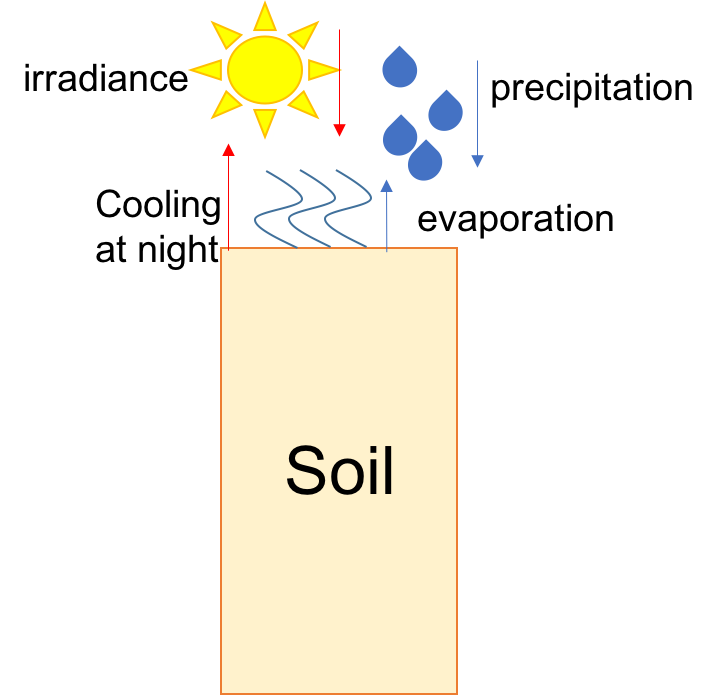
\includegraphics[width=8cm]{coupled.png}
\caption{Simplified scheme of coupled model.}
\end{figure}

In the real world many coupled processes occur. Heat conduction is dependent on the water content and water flow is dependent on heat properties. 

In this tutorial three configuration files will be modified step by step. All configuration files are located in the folder \emph{drutes.conf} and respective subfolders. \begin{enumerate}
\item For selection of the module, dimension and time information we require \emph{global.conf}.  \emph{global.conf} is located in \emph{drutes.conf / global.conf}. 
\item To define the mesh or spatial discretization in 1D,  we require \emph{drumesh1D.conf}. \emph{drumesh1D.conf} is located in \emph{drutes.conf / mesh / drumesh1D.conf}. 
\item To define the radiation and cooling, we require \emph{matrix.conf}. \emph{matrix.conf} is located in \emph{drutes.conf /water.conf/ matrix.conf}. 
\end{enumerate}
\item To define the precipitation and evaporation, we require \emph{matrix.conf}. \emph{matrix.conf} is located in \emph{drutes.conf /water.conf/ matrix.conf}. 
\end{enumerate}
$DRUtES$ works with configuration input file with the file extension .conf. Blank lines and lines starting with \# are ignored. The input mentioned in this tutorial therefore needs to be placed one line below the mentioned keyword, unless stated otherwise. 

\section{Software}

\begin{enumerate}
\item Install $DRUtES$. You can get $DRUtES$ from the github repository \href{https://github.com/michalkuraz/drutes-dev/} {drutes-dev} or download it from the \href{http://drutes.org/public/?core=account}{drutes.org} website. 
\item Follow website instructions on \href{http://drutes.org/public/?core=account}{drutes.org} for the installation.
\item Working R installation (optional, to generate plots you can execute freely distributed R script) 
\end{enumerate}

\newpage
\section{Scenarios}

We are using the well-known van Genuchten-Mualem parameterization to describe the soil hydraulic properties of our soils. 

\begin{table}[!h]
\centering
\caption{\label{tab_heat}Material properties needed for scenarios.}
\adjustbox{max height=\dimexpr\textheight-2cm\relax,
           max width=\textwidth}{

\small\begin{tabular}{l l c c }
\hline
Parameter & Description & Soil \\
\hline

$\alpha$ [cm$^{-1}$]& inverse of the air entry value &0.05 \\
 $n$ [-]& shape parameter &2 \\
 $m$ [-]& shape parameter &0.5  \\
  $ \theta_s$ [-]&saturated vol. water content&0.45 \\
  $ \theta_r$ [-]& residual vol. water content&0.05  \\
  $Ss$ [cm$^{-1}$] & specific storage & 0 \\
  $K_s$ [cm d$^{-1}$] & saturated hydraulic conductivity & 100 \\ 
\hline
\end{tabular}
}
\end{table}
\begin{figure}[!h]


\begin{figure}[!h]
\centering
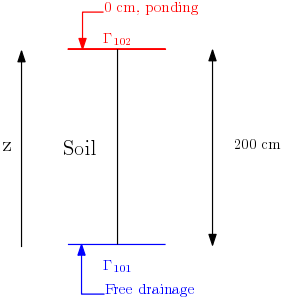
\includegraphics[width=5cm]{domain.png}
\caption{1D domain set-up of infiltration scenario with top and bottom boundary conditions. A constant ponding is assigned to the top, defined with a Dirichlet condition of 0 cm. Free drainage occurs at the bottom, which indicates that the pressure head gradient is 0 and water flows only due to gravity.}
\end{figure}

\newpage

\section*{Scenario 1}

Infiltration into sandy soil. 

$global.conf$: Choose correct model, dimension, time discretization and observation times.
\begin{enumerate}
\item Open \textbf{\emph{global.conf}} in a text editor of your choice. 
\item Model type: Your first input is the module. Input is \textbf{RE}.
\item Initial mesh configuration \begin{enumerate}
\item The dimension of our problem is 1. Input: 1.
\item We use the internal mesh generator. Input: 1. 
\end{enumerate}
\item Error criterion \begin{enumerate} 
\item Maximum number of iteration of the Picard method: 20 
\item h tolerance: 1e-1.
\end{enumerate}
\item Time information 
\begin{enumerate} 
%\item integration method is 3 point formula. Input: 30. 
\item Time units are in hours: input d
\item Initial time: 1e-4.
\item End time: 1.
\item Minimum time step: 1e-4.
\item Maximum time step: 0.1.
\end{enumerate}
\item Observation time settings \begin{enumerate}
\item Observation time method: 2
\item Set file format of observation: pure. Output in 1D is always in raw data. Different options will not impact output in 1D.
\item Make sequence of observation time: n
\item Number of observation times: 10
\item Observation time values: 0.001,
0.005,
0.01,
0.05,
0.1,
0.2,
0.3,
0.4,
0.6,
0.8. Use a new line for each input. \textit{DRUtES} automatically generates output for the initial time and final time. DRUtES will generate 12 output files, e.g. \textit{RE\_matrix\_press\_head-x.dat}, \textit{RE\_matrix\_theta-x.dat} where x is the number of the file and not the output time. The initial time is assigned an x value of 0. 
\end{enumerate}
\item Observation point settings \begin{enumerate}
\item Observation point coordinates: 0, 200. Use a new line for each input. \textit{DRUtES} will generate 2 output files, e.g. \textit{obspt\_RE\_matrix-1.out}, where x is the ID of the observation point. 
\end{enumerate}
\item Ignore other settings for now. 
\item Save $global.conf$
\end{enumerate}


$drumesh1D.conf$: Mesh definition, i.e. number of materials and spatial discretization
\begin{enumerate}
\item Open \textbf{\emph{drumesh1D.conf}} in a text editor of your choice. 
\item Geometry information: 200 cm - domain length
\item Amount of intervals: 1
\item
\adjustbox{max height=\dimexpr\textheight-5cm\relax,
           max width=\textwidth}{
\small\begin{tabular}{|c | c | c|}
\hline
density & bottom & top \\
 \hline
5 & 0 & 200\\
\hline
\end{tabular}
}
\item number of materials: 1
\item \adjustbox{max height=\dimexpr\textheight-5cm\relax,
           max width=\textwidth}{
\small\begin{tabular}{|c | c | c|}
\hline
id & bottom & top \\
 \hline
5 & 0 & 200 \\
\hline
\end{tabular}
}
\end{enumerate}

\emph{matrix.conf}: Configuration file for water flow 


\begin{enumerate}
\item Open \emph{matrix.conf} in a text editor of your choice. 
\item How-to use constitutive relations? [integer]: 1
\item Length of interval for precalculating the constitutive functions: 200
\item Discretization step for constituitive function precalculation: 0.1
\item number of soil layers [integer]: 1
\item \adjustbox{max height=\dimexpr\textheight-5cm\relax,
	max width=\textwidth}{
	\small\begin{tabular}{|c | c | c|c | c | c|}
		\hline
		alpha & n & m & theta\_r & theta\_s & specific storage\\
		\hline
		0.1 & 2.2  & 0.55 & 0.00 & 0.40  &0  \\
		\hline
	\end{tabular}
}
\item The angle of the anisotropy determines the angle of the reference coordinate system. 0 means vertical flow. Anisotropy description. Anisotpropy description and hydraulic conductivity\\ \adjustbox{max height=\dimexpr\textheight-5cm\relax,
	max width=\textwidth}{
	\small\begin{tabular}{|c | c |}
		\hline
		angle [degrees] & K\_11  \\
		\hline
		0 & 400  \\
		\hline
	\end{tabular}
}
\item sink(-) /source (+) term per layer: 0
\item Initial condition is a constant pressure head of -200 cm across the soil. \adjustbox{max height=\dimexpr\textheight-5cm\relax,
	max width=\textwidth}{
	\small\begin{tabular}{|c | c | c|c |}
		\hline
		 init. cond [real] & type of init. cond &RCZA method [y/n] &  RCZA method val.  \\
		\hline
		   -200.0           &            hpres                       & n		   &          0 \\
		\hline
	\end{tabular}
}
\item number of boundaries: 2
\item \adjustbox{max height=\dimexpr\textheight-5cm\relax,
	max width=\textwidth}{
	\small\begin{tabular}{|c | c | c|c |}
		\hline
		boundary ID& boundary type   & use rain.dat [y/n]   & value  \\
		\hline
	101    &                   3        &           n        &        0.0 \\
	102             &          1         &          n         &       0.0        \\
	
		\hline
	\end{tabular}
}
\item Save matrix.conf.

\end{enumerate}

\section*{Run scenario 1}
Run the simulation in the terminal console.
\begin{enumerate}
\item Make sure you are in the right directory. 
\item To execute $DRUtES$: \\
\$ bin/drutes
\item After the simulation finishes, to generate png plots execute provided R script: \\
\$ Rscript drutes.conf/water.conf/waterplots.R -name sand
\item The output of the simulation can be found in the folder out
\end{enumerate}

\section*{Scenario 2}
Infiltration into silty soil
\begin{enumerate}
\item \emph{global.conf} and \emph{drumesh1D.conf} remain the same.
\item Open \emph{matrix.conf} in a text editor of your choice. 
\item Use the same set-up, but change the van Genuchten parameters to:
\item \adjustbox{max height=\dimexpr\textheight-5cm\relax,
	max width=\textwidth}{
	\small\begin{tabular}{|c | c | c|c | c | c|}
		\hline
		alpha & n & m & theta\_r & theta\_s & specific storage\\
		\hline
		0.08 & 1.8   & 0.44 & 0.05 & 0.45  & 0 \\
		\hline
	\end{tabular}
}
\item anisothprophy description and hydraulic conductivity\\ \adjustbox{max height=\dimexpr\textheight-5cm\relax,
	max width=\textwidth}{
	\small\begin{tabular}{|c | c |}
		\hline
		angle [degrees] & K\_11  \\
		\hline
		0 & 40  \\
		\hline
	\end{tabular}
}
\item Save matrix.conf.
\end{enumerate}

\section*{Run scenario 2}
Run the simulation in the terminal console.
\begin{enumerate}
\item To execute $DRUtES$: \\
\$ bin/drutes
\item generate png plots with R script: \\
\$ Rscript drutes.conf/water.conf/waterplots.R -name silt
\end{enumerate}

\section*{Scenario 3}
Infiltration into clay soil
\begin{enumerate}
\item \emph{global.conf} and \emph{drumesh1D.conf} remain the same.
\item Open \emph{matrix.conf} in a text editor of your choice. 
\item Use the same set-up, but change the van Genuchten parameters to:
\item \adjustbox{max height=\dimexpr\textheight-5cm\relax,
	max width=\textwidth}{
	\small\begin{tabular}{|c | c | c|c | c | c|}
		\hline
		alpha & n & m & theta\_r & theta\_s & specific storage\\
		\hline
		0.01 & 1.5  & 0.33 & 0.1& 0.5   &0 \\
		\hline
	\end{tabular}
}
\item anisothprophy description and hydraulic conductivity\\ \adjustbox{max height=\dimexpr\textheight-5cm\relax,
	max width=\textwidth}{
	\small\begin{tabular}{|c | c |}
		\hline
		angle [degrees] & K\_11  \\
		\hline
		0 & 4  \\
		\hline
	\end{tabular}
}
\item Save matrix.conf.
\end{enumerate}

\section*{Run scenario 3}
Run the simulation in the terminal console.
\begin{enumerate}
\item To execute $DRUtES$: \\
\$ bin/drutes
\item generate png plots with R script: \\
\$ Rscript drutes.conf/water.conf/waterplots.R -name clay
\end{enumerate}

\section*{Tasks}

\begin{enumerate}
\item Describe the infiltration fronts for sand, silt and clay.
\item The results do not look very smooth. This is because of insufficient discretization. Improve the discretization for sand. With what set-up are the results better? Possibilities are: 
\begin{itemize}
\item in global.conf: Decrease the pressure head tolerance, Decrease the initial time step, Decrease the maximum time step.
\item in drumesh1D.conf: Decrease the mesh density. 
\end{itemize}
\item Why is the flux at the top so huge in the beginning?
\end{enumerate}



\section*{Results}

\subsection*{Task 1}
In the following time series of the infiltration into sand, silt and clay are presented. The infiltration front has moved furthest in sand, followed by silt and then clay. This is because of the assigned boundary conditions. The flux into sandy soil is very large. However, the time series show the numerical approximation is insufficient, especially for sand. This is because sand is the numerically most difficult to model as it has the steepest retention properties (largest n and largest alpha).

\begin{figure}[!h]
\centering
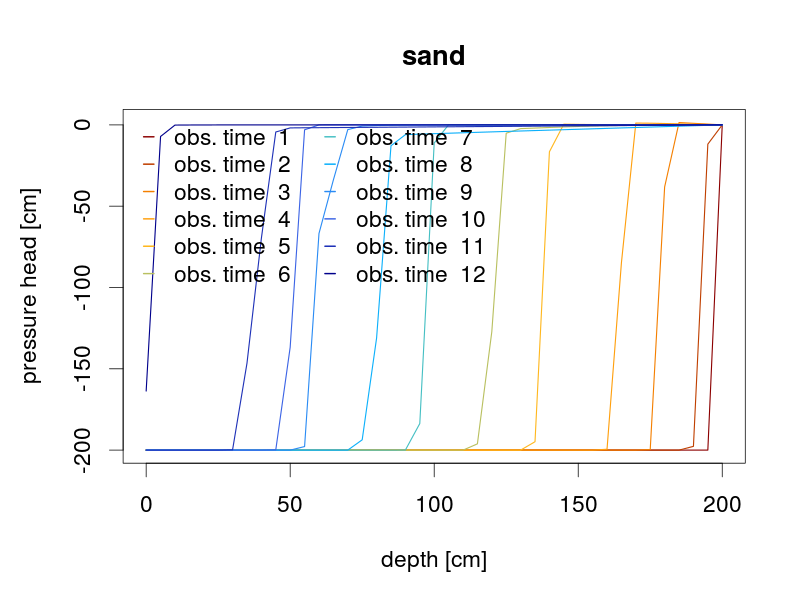
\includegraphics[width=0.49\textwidth]{obs_press_head_sand.png}
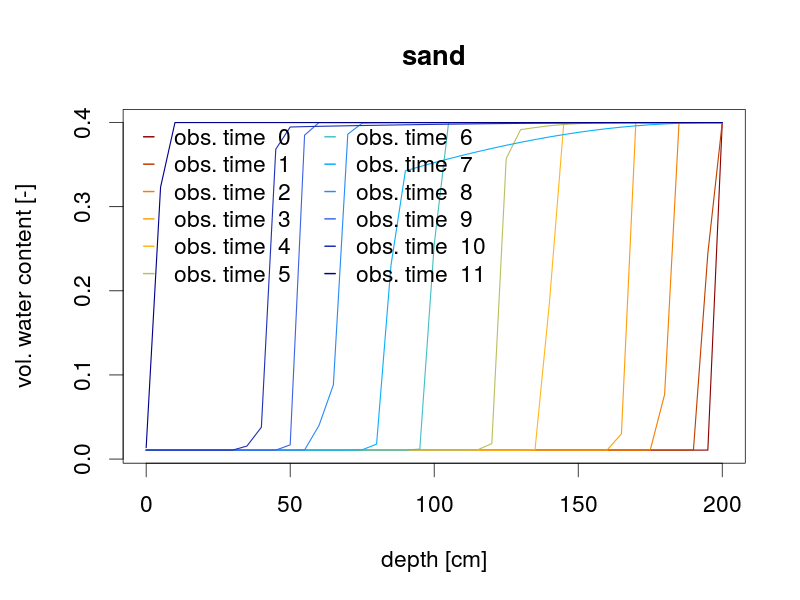
\includegraphics[width=0.49\textwidth]{obs_water_sand.png}
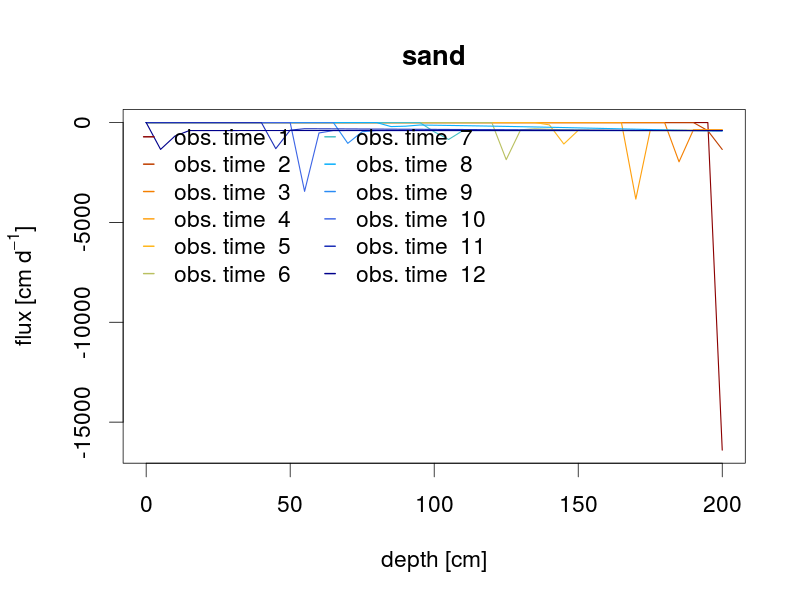
\includegraphics[width=0.49\textwidth]{obs_flux_sand.png}
\caption{Observation time series of pressure head, vol. water content and flux of infiltration into sand.}
\end{figure}

\begin{figure}[!h]
\centering
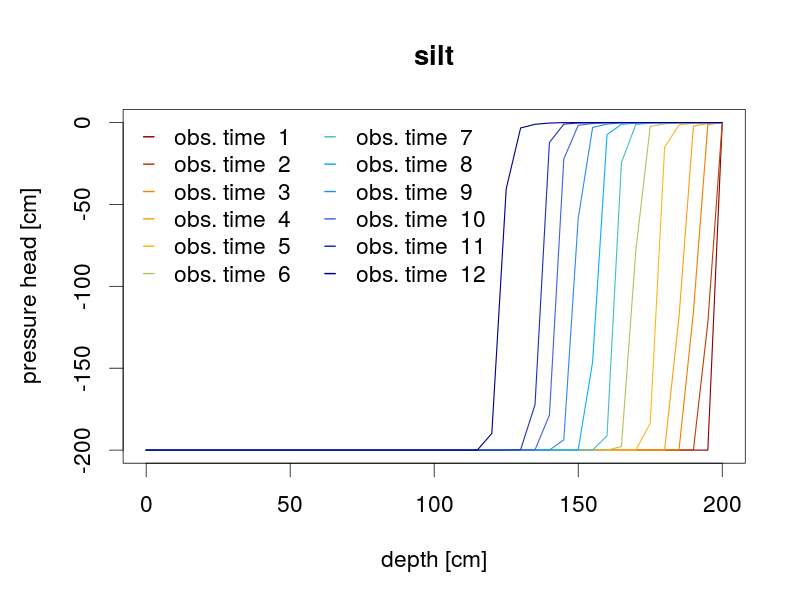
\includegraphics[width=0.49\textwidth]{obs_press_head_silt.png}
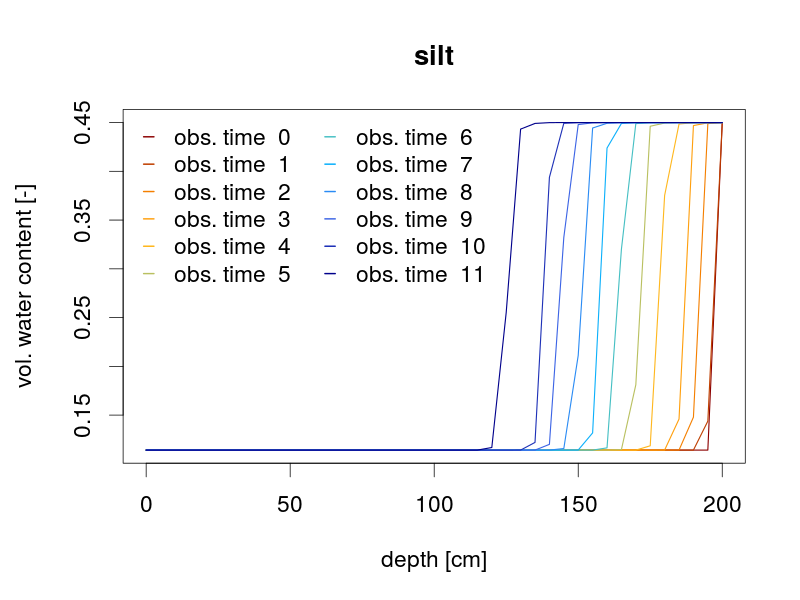
\includegraphics[width=0.49\textwidth]{obs_water_silt.png}
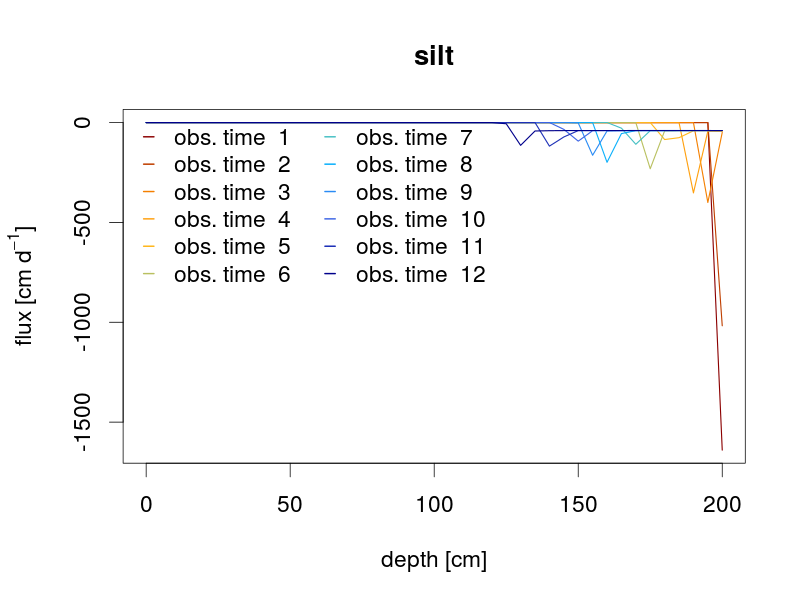
\includegraphics[width=0.49\textwidth]{obs_flux_silt.png}
\caption{Observation time series of pressure head, vol. water content and flux of infiltration into silt.}

\end{figure}


\begin{figure}[!h]
\centering
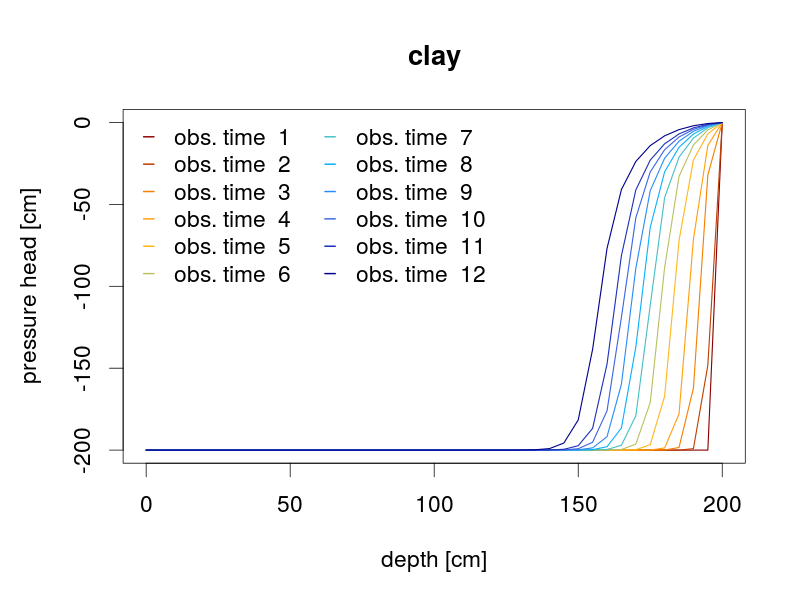
\includegraphics[width=0.49\textwidth]{obs_press_head_clay.png}
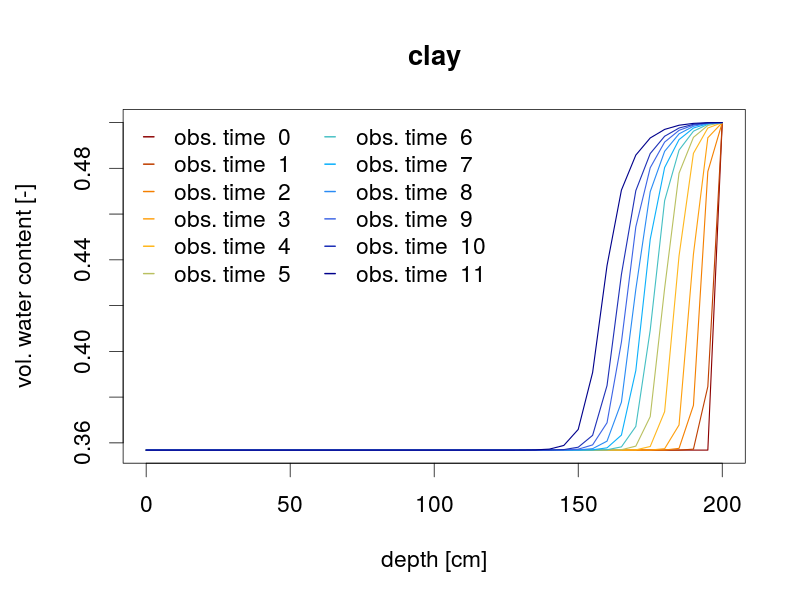
\includegraphics[width=0.49\textwidth]{obs_water_clay.png}
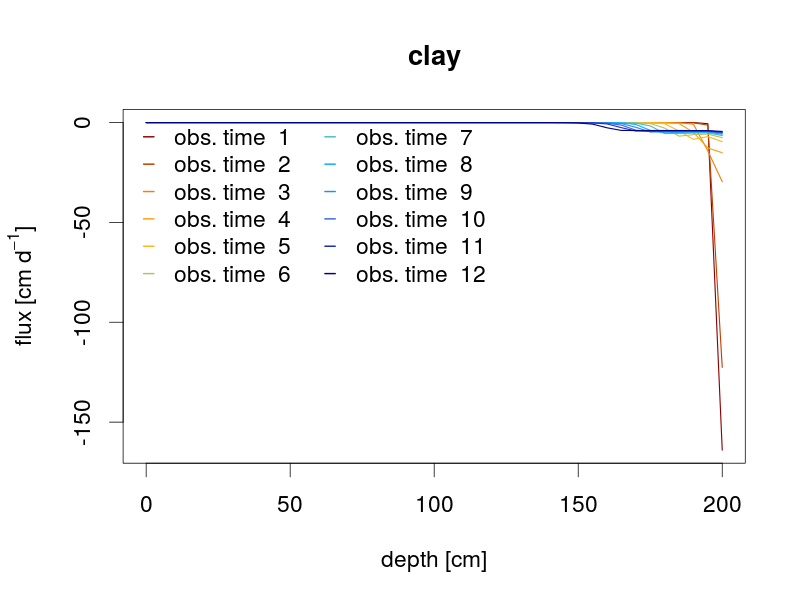
\includegraphics[width=0.49\textwidth]{obs_flux_clay.png}
\caption{Observation time series of pressure head, vol. water content and flux of infiltration into clay.}

\end{figure}

\newpage
\newpage
\subsection*{Task 2}

The solution for sand the water content and hydraulic pressure become a lot smoother with finer spatial discretization, eg. dz=0.5 and a finer temporal discretization by setting the lower minimal time step to 0.01. The fluxes are still spiky, but correlate with the infiltration front. Different solutions can be found by decreasing the minimal time step even further and also the h tolerance criterion. This, however, increases the simulation time substantially. For a reliable solution, the numerical solution should converge. This means that decreasing the time step, or discretization, should not lead to an entirely different solution. We notice, that reducing the h tolerance criterion improves the solution locally, but that reducing the maximum time step changes the depth of the infiltration front. This is because the mass balance is very much connected to the temporal discretization.

\begin{figure}[!h]
	\centering
	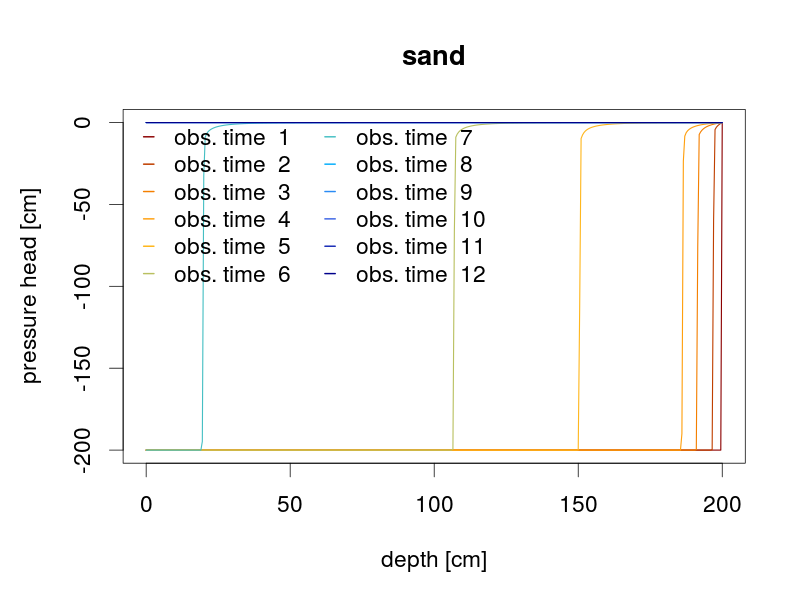
\includegraphics[width=0.49\textwidth]{obs_press_head_sand6.png}
	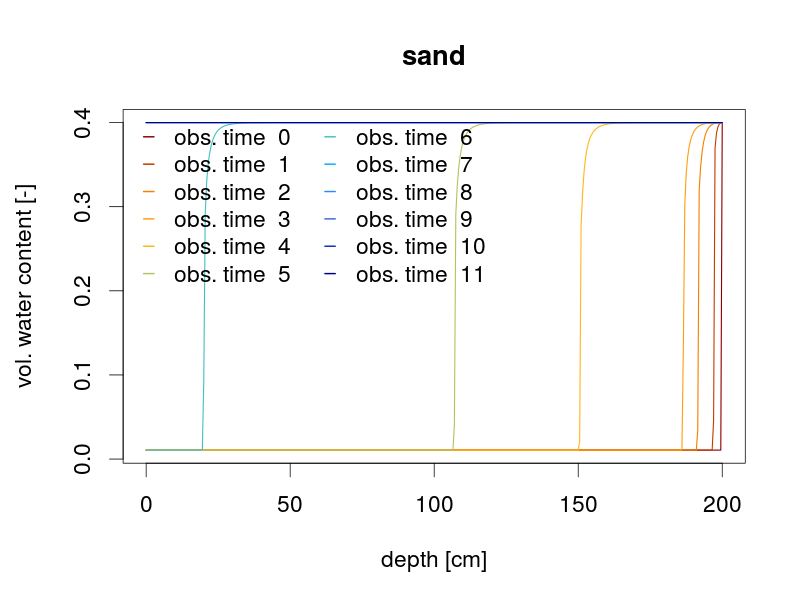
\includegraphics[width=0.49\textwidth]{obs_water_sand6.png}
	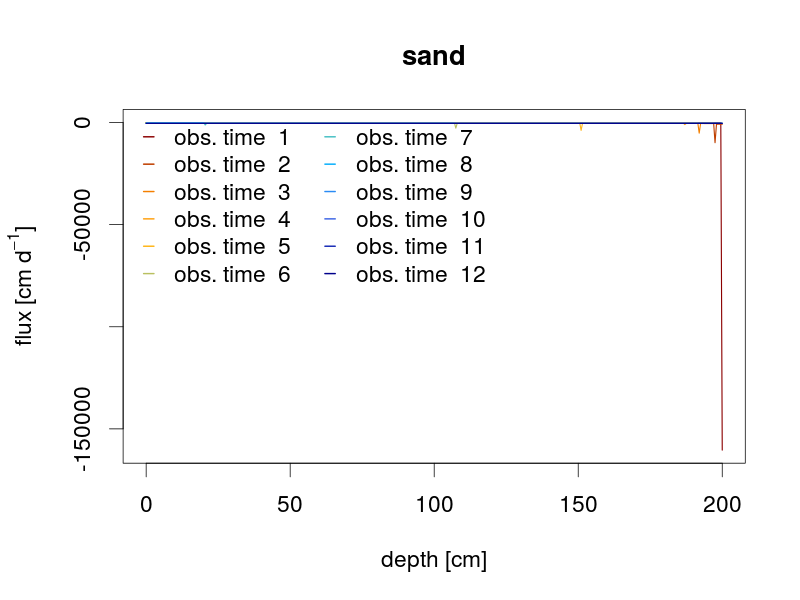
\includegraphics[width=0.49\textwidth]{obs_flux_sand6.png}
	\caption{Observation time series of pressure head, vol. water content and flux of infiltration into sand with improved discretization.}
\end{figure}

\subsection*{Task 3}
With the initial set-up, the flux at the top in sand is 15000 cm d$^{-1}$ in the beginning of the simulation. For silt, the flux was numerically calculated to be at 1500 cm d$^{-1}$ and for clay at 150 cm d$^{-1}$. The flux estimation becomes a lot larger with finer spatial discretization.

 This is due to the large hydraulic gradient between the saturated top boundary and the next node of $\nabla h=\frac{-200-0~}{\mathrm{dz}}$. The smaller the nodal distance dz is, the greater is the gradient. According to the Darcy-Buckingham law, the flux is proportional to the hydraulic conductivity. The hydraulic conductivity is highest for sand. This is why the flux is largest for sand and lowest for clay.
\newpage
\newpage
\newpage
\newpage
\section{Outcome}
\begin{enumerate}
\item You got familiar with the $DRUtES$ standard Richards Equation modules in 1D.
\item You understand basic parameterization of a typical sand, silt and clay with the van Genuchten-Mualem model.
\item You simulated infiltration in different soils.
\item You understand the term \emph{Free drainage} and \emph{initial condition}.
\item You understand the effects of different discretizations.
\end{enumerate}



%----------------------------------------------------------------------------------------
%	BIBLIOGRAPHY
%----------------------------------------------------------------------------------------

%\renewcommand{\refname}{\spacedlowsmallcaps{References}} % For modifying the bibliography heading

%\bibliographystyle{unsrt}

%\bibliography{sample.bib} % The file containing the bibliography

%----------------------------------------------------------------------------------------

\end{document}